\documentclass[10pt,twocolumn]{article}
\usepackage[margin=0.75in]{geometry}
\usepackage{times}
\usepackage{graphicx}
\usepackage{booktabs}
\usepackage{amsmath,amssymb}
\usepackage{url}
\usepackage{hyperref}
\usepackage[numbers,sort&compress]{natbib}

\title{Dual-Regime Insert/Abort:\\
Sensor Perturbation vs.\ Selection Shift}
\author{Ruililin Shen\\
\texttt{bobshenruililin@gmail.com}}
\date{31 August 2026}

% Auto-generated by scripts/make_paper_numbers.py from results/*.json.
% Do not edit by hand.
\newcommand{\NumExpFourN}{240}
\newcommand{\NumExpFourFailed}{0}
\newcommand{\NumExpFourSeconds}{23.0}
\newcommand{\NumNoneDeltaMean}{0.113}
\newcommand{\NumNoneDeltaStd}{0.149}
\newcommand{\NumNoneNPos}{51}
\newcommand{\NumNoneNNeg}{9}
\newcommand{\NumNoneN}{60}
\newcommand{\NumTempDeltaMean}{0.124}
\newcommand{\NumTempDeltaStd}{0.150}
\newcommand{\NumIsoDeltaMean}{0.141}
\newcommand{\NumIsoDeltaStd}{0.151}
\newcommand{\NumHistDeltaMean}{0.141}
\newcommand{\NumHistDeltaStd}{0.151}
\newcommand{\NumNonePooledP}{2.2e-10}
\newcommand{\NumTempPooledP}{3.1e-11}
\newcommand{\NumIsoPooledP}{4.6e-11}
\newcommand{\NumHistPooledP}{3.3e-11}
\newcommand{\NumBcLogregAcc}{0.979}
\newcommand{\NumBcLogregEce}{0.032}
\newcommand{\NumBcLogregEceStd}{0.010}
\newcommand{\NumWineRfEceIid}{0.147}
\newcommand{\NumWineRfEceIidStd}{0.020}
\newcommand{\NumWineLogregAcc}{0.982}
\newcommand{\NumBcHgbDelta}{0.002}
\newcommand{\NumBcHgbDeltaStd}{0.009}
\newcommand{\NumSynthLogregDelta}{0.292}
\newcommand{\NumSynthLogregDeltaStd}{0.214}
\newcommand{\NumBcLogregCovSZero}{0.913}
\newcommand{\NumBcLogregCovSOneFive}{0.778}
\newcommand{\NumBcLogregCovSTwoFive}{0.608}
\newcommand{\NumSynthLogregCovSOneFive}{0.634}
\newcommand{\NumWineRfIsoHelp}{-0.123}
\newcommand{\NumBcLogregIsoHelp}{0.074}
\newcommand{\NumWineRfTempSh}{0.068}
\newcommand{\NumWineRfNoneSh}{0.175}
\newcommand{\NumTempNPos}{56}
\newcommand{\NumTempNNeg}{4}
\newcommand{\NumIsoNPos}{53}
\newcommand{\NumIsoNNeg}{7}
\newcommand{\NumHistNPos}{57}
\newcommand{\NumHistNNeg}{3}
\newcommand{\NumNoiseSynthRf}{0.009}
\newcommand{\NumPredSynthRf}{0.041}
\newcommand{\NumNSeeds}{5}
\newcommand{\NumAlpha}{0.1}
\newcommand{\NumEceBins}{15}
\newcommand{\NumNTests}{22}
\newcommand{\NumTwelveMeanP}{2.4e-04}
\newcommand{\NumTwelveMeanNPos}{12}
\newcommand{\NumTwelveMeanN}{12}
\newcommand{\NumQuantileSliceDeltaMean}{0.016}
\newcommand{\NumQuantileSliceDeltaStd}{0.006}
\newcommand{\NumImpResampleDeltaMean}{0.011}
\newcommand{\NumImpResampleDeltaStd}{0.031}
\newcommand{\NumSynthLogregAccIid}{0.932}
\newcommand{\NumSynthLogregAccShifted}{0.620}
\newcommand{\NumSklearnDeltaMean}{0.042}
\newcommand{\NumSklearnDeltaStd}{0.039}
\newcommand{\NumSklearnNPos}{25}
\newcommand{\NumSklearnNNeg}{5}
\newcommand{\NumSklearnN}{30}
\newcommand{\NumSynthDeltaMean}{0.184}
\newcommand{\NumSynthDeltaStd}{0.183}
\newcommand{\NumSynthNPos}{26}
\newcommand{\NumSynthNNeg}{4}
\newcommand{\NumSynthN}{30}
\newcommand{\NumNoneDeltaAccMean}{-0.156}
\newcommand{\NumNoneDeltaBrierMean}{0.257}
\newcommand{\NumNoneDeltaNllMean}{0.792}
\newcommand{\NumWineRfIsoSh}{0.052}
\newcommand{\NumExpFiveN}{6}
\newcommand{\NumExpFiveNDs}{2}
\newcommand{\NumMatchedGaussDeltaMean}{0.105}
\newcommand{\NumMatchedGaussDeltaStd}{0.109}
\newcommand{\NumQuantileDeltaAccMean}{-0.016}
\newcommand{\NumMatchedGaussDeltaAccMean}{-0.128}
\newcommand{\NumWineNTest}{45}
\newcommand{\NumWineNCal}{44}
\newcommand{\NumBcLogregCovSZeroStd}{0.015}
\newcommand{\NumBcLogregCovSOneFiveStd}{0.045}
\newcommand{\NumSynthLogregCovSOneFiveStd}{0.190}
\newcommand{\NumDatasetSignP}{0.0625}
\newcommand{\NumDatasetSignN}{4}
\newcommand{\NumPertRouterUtil}{0.093}
\newcommand{\NumPertIidUtil}{-3.000}
\newcommand{\NumPertAbortUtil}{-0.500}
\newcommand{\NumPertIllegalUtil}{-3.000}
\newcommand{\NumPertDenoiseOffUtil}{-0.500}
\newcommand{\NumPertRouterFcr}{0.014}
\newcommand{\NumPertIidFcr}{0.342}
\newcommand{\NumPertIllegalFcr}{0.342}
\newcommand{\NumPertRouterRec}{0.826}
\newcommand{\NumPertRouterAct}{0.396}
\newcommand{\NumPertRouterAbort}{0.110}
\newcommand{\NumSelRouterAbort}{0.000}
\newcommand{\NumSelRouterUtil}{0.158}
\newcommand{\NumSelAbortUtil}{-0.500}
\newcommand{\NumIidRouterUtil}{0.177}
\newcommand{\NumIidIidUtil}{0.176}
\newcommand{\NumDualNSeeds}{5}
\newcommand{\NumDualPosIid}{0.458}
\newcommand{\NumDualPosSel}{0.426}
\newcommand{\NumDualKillsFired}{none}
\newcommand{\NumPertOracleUtil}{0.126}
\newcommand{\NumPertProjectUtil}{0.126}
\newcommand{\NumStreamPertPredP}{0.929}
\newcommand{\NumStreamSelPredS}{0.949}
\newcommand{\NumStreamPertProj}{0.804}


\begin{document}
\maketitle
\begin{abstract}
Temperature scaling and related post-hoc maps are often treated as a cheap
fix for miscalibrated probabilities. We measure whether that fix
transfers under two different test-time changes, for logistic regression,
random forests, and histogram gradient boosting on small tabular datasets
(no deep nets, no API models). \emph{Feature mean-shift with frozen
labels}---a perturbation of $X$ that does \textbf{not} preserve
$P(Y\mid X)$---raises ECE: at strength $1.5$, uncalibrated
$\Delta\mathrm{ECE}=\mathrm{ECE}_{\mathrm{pert}}-\mathrm{ECE}_{\mathrm{iid}}$
is positive in \NumNoneNPos/\NumNoneN{} seed-level cells (mean
\NumNoneDeltaMean, cell-to-cell sd \NumNoneDeltaStd). That pool mixes
sklearn sets (mean \NumSklearnDeltaMean,
\NumSklearnNPos/\NumSklearnN{} positive) with synthetics (mean
\NumSynthDeltaMean, \NumSynthNPos/\NumSynthN{} positive) where accuracy
also falls. Averaging seeds first, all
\NumTwelveMeanNPos/\NumTwelveMeanN{} uncalibrated
dataset$\times$model means are positive (a sign count; models that share
a dataset are not independent). After i.i.d.\ temperature, isotonic, or
histogram maps, pooled $\Delta\mathrm{ECE}$ remains positive. The same
maps can help or hurt relative to doing nothing. By contrast,
\emph{selection} on $X$ that keeps the original $(X,y)$ pairs---closer
to covariate shift, but a milder change in accuracy---yields smaller
$\Delta\mathrm{ECE}$ (quantile-slice cell-mean
\NumQuantileSliceDeltaMean{} on \NumExpFiveN{} dataset$\times$model cells
from \NumExpFiveNDs{} datasets). Unweighted split-conformal coverage
falls under feature perturbation. On a planar peg-in-hole
\emph{insert vs.\ abort} cartoon (geometric clearance, not a robot), an
optimistic encoder---frozen labels, reports the peg closer to the hole
than the true pose---makes source temperature on \emph{raw} encoder
probabilities a false-confident insert policy (FCAR
\NumPertIllegalFcr, mean utility \NumPertIllegalUtil). A physics-residual
channel that \emph{projects} the encoder onto the camera pose and only
then applies the same source $T$ recovers utility \NumPertRouterUtil{}
(FCAR \NumPertRouterFcr, \NumDualNSeeds{} seeds) and beats abort-all
(\NumPertAbortUtil). A pairing-preserving fixture slice is
difficulty-matched (success rate \NumDualPosSel{} vs.\ i.i.d.\
\NumDualPosIid) and is not aborted as a sensor fault (abort rate
\NumSelRouterAbort). This is an analysis-plus-system result, not a new
calibrator and not hardware.
\end{abstract}

\section{Introduction}
A classifier is \emph{calibrated} when a predicted probability $p$ is
correct with frequency $p$. Post-hoc maps---Platt-style scaling, histogram
binning, isotonic regression, and temperature scaling---are the standard
way to improve calibration without retraining
\cite{zadrozny2002multiclass,niculescumizil2005probabilities,guo2017calibration}.
A separate literature shows that deep-net uncertainty \emph{collapses}
under dataset shift \cite{ovadia2019trust,minderer2021revisiting,tomani2021posthoc}.
Almost all of that evidence is vision-scale neural nets. Tree ensembles
remain strong on tabular data \cite{grinsztajn2022trees}, and their
i.i.d.\ calibration properties have been known for decades
\cite{niculescumizil2005probabilities}. Within our API-verified bibliography---mostly deep-net calibration and
conformal theory, not a systematic search of applied tabular-drift
venues---we did not find this exact measurement (sklearn models, i.i.d.\ post-hoc maps, test-time
feature perturbation vs.\ selection). That is a scoped gap, not a proof
of absence.

We treat that as a measurement question. We do not introduce a new
calibrator. A negative or mixed answer is an acceptable outcome.

\paragraph{Primary hypothesis (reframed).}
I.i.d.-fitted post-hoc maps do not keep ECE from rising under a Gaussian
mean-shift of test features with \emph{labels held fixed} (input
perturbation / a change in $P(Y\mid X)$ at the observed $x$). We do
\textbf{not} claim that genuine covariate shift---selection on $X$ that
preserves pairings---has the same effect; that is tested as a control.

Two other hypotheses were piloted and \emph{not} selected as the paper
claim: isotonic overfit vs.\ temperature as a function of $n_{\mathrm{cal}}$
(H2; heterogeneous), and oracle-weighted conformal recovery (H3; the 1-D
weight estimator failed). Decision log: \texttt{logs/decisions.md}.

\section{Related work}
Surveys of calibration methods and metrics include
\cite{silvafilho2021survey,wang2023survey}.
ECE via confidence binning \cite{naeini2015bbq,guo2017calibration} is
biased and definition-dependent
\cite{nixon2019measuring,kumar2019verified,vaicenavicius2019evaluating};
we therefore also report Brier score \cite{brier1950verification} and
NLL \cite{gneiting2007scoring} (pooled $\Delta$ alongside ECE in
Results). Temperature scaling
\cite{guo2017calibration} and Dirichlet calibration
\cite{kull2019dirichlet} target neural nets. Unsupervised recalibration
under covariate shift exists for neural models
(Pampari and Ermon~\cite{pampari2020unsupervised}). Domain-drift post-hoc
calibration of CNNs is studied by Tomani et~al.~\cite{tomani2021posthoc}.
Those papers already
\textit{predict} our headline outcomes: ECE should rise under shift, and
i.i.d.-fitted post-hoc maps should not be a complete fix. A surprising
result here would have been that logistic regression, random forests, and
histogram boosting \emph{stay} calibrated under a mean-shift of used
covariates \emph{with labels frozen}. Selection that preserves
$(X,y)$ pairs is a different mechanism. We reuse the questions, not the
model class.

Conformal prediction has finite-sample coverage under exchangeability
\cite{vovk2005algorithmic,lei2016distributionfree,angelopoulos2021gentle}
and requires density-ratio weights under covariate shift
\cite{tibshirani2019covariate}. We use unweighted split conformal as a
secondary diagnostic, not as a proposed fix.
Conformal warning systems for grasping and driving
\cite{luo2021conformal} and perception-based safe control
\cite{yang2023safeperception,huang2023conformalpolicy} treat shift as
one blob. Density-ratio conformal \cite{tibshirani2019covariate} is the
legal act policy only while $P(Y\mid X)$ is invariant, which frozen-label
encoder bias violates. We do not claim a method gap versus those papers.
The system question here is whether unlabeled residual vs.\ density
channels can route \emph{opposite} legal moves on a DGP where those
assumptions split.

\section{Methods}
\paragraph{Models.}
Scikit-learn logistic regression (with standard scaling), random forests,
and \texttt{HistGradientBoostingClassifier}, with hyperparameters as in
\texttt{src/calibshift/models.py}. All expose \texttt{predict\_proba}.

\paragraph{Calibrators.}
Fitted on a held-out calibration split of the \emph{source} distribution,
then frozen. \texttt{none}: identity. \texttt{temperature}: one scalar
$T$ on $\log p$, fitted by NLL (Guo-style, using log-probabilities so
trees without logits still apply). \texttt{isotonic}: sklearn isotonic
regression on $p(y{=}1)$ (binary) or on confidence (multiclass).
\texttt{histogram}: equal-width binning of the same 1-D score.

\paragraph{Shifts.}
\textit{Feature perturbation:} add $s\cdot\hat\sigma_j$ to listed test
columns, \textbf{keeping the original labels}. This moves $x$ without
moving $y$, so it is \emph{not} covariate shift ($P(Y\mid X)$ is not
invariant). $\hat\sigma$ is the test-split feature sd.
\textit{Selection:} quantile slice and importance resampling of existing
$(X,y)$ pairs (closer to covariate shift). Trailing-column perturbation
is a control.

\paragraph{Metrics.}
Equal-width confidence ECE with \NumEceBins{} bins (from the exp04
config), Brier, NLL, accuracy, and split conformal coverage with the
inverse-probability (LAC) score $1-p_y$ at $\alpha=\NumAlpha$
(not APS).

\paragraph{Protocol.}
Train/calibration/test partitions follow \texttt{calibshift.runner}
(source-distribution splits; calibration data never includes the test
set), stratified, with the \NumNSeeds{} seeds listed in the exp04 config.
Results are written only by \texttt{calibshift.io.write\_result}.
\texttt{paper/numbers.tex} is generated from those JSON files.

\section{Experiments}
\paragraph{Datasets.}
Offline-only: sklearn \texttt{breast\_cancer} (binary) and \texttt{wine}
(3-class); two \texttt{make\_classification} sets (binary and 3-class).
No OpenML, no paid APIs.

\paragraph{Main grid (\texttt{exp04\_main\_h1}).}
\NumExpFourN{} cells, \NumExpFourFailed{} failed, \NumExpFourSeconds{}
seconds on CPU. This is the source of all headline numbers.

\paragraph{Ablations.}
\texttt{exp05}: quantile slice and importance resampling.
\texttt{exp06}: calibration-set size (killed primary H2).
\texttt{exp07}: shift trailing columns.

\paragraph{Sanity.}
I.i.d.\ logistic regression on breast-cancer: accuracy \NumBcLogregAcc,
ECE \NumBcLogregEce$\pm$\NumBcLogregEceStd (linear models on this set
are typically $\gtrsim 0.95$ accurate). Wine random forests are
overconfident i.i.d.\ (ECE \NumWineRfEceIid$\pm$\NumWineRfEceIidStd),
matching the classical tree-calibration picture
\cite{niculescumizil2005probabilities}. Split conformal coverage at
$s{=}0$ is near the nominal $1-\alpha=0.9$ for $\alpha{=}\NumAlpha$. We do \emph{not} compare
ECE magnitudes to ImageNet temperature scaling \cite{guo2017calibration}.

\section{Results}
\subsection{Feature perturbation usually raises ECE}
Figure~\ref{fig:ece} plots shifted ECE against perturbation strength $s$.
Figure~\ref{fig:heat} shows mean $\Delta\mathrm{ECE}$ at $s{=}1.5$.
Pooled over \NumNoneN{} dataset$\times$model$\times$seed cells,
uncalibrated mean $\Delta\mathrm{ECE}=\NumNoneDeltaMean$ with
cell-to-cell sd \NumNoneDeltaStd{}
(\NumNoneNPos{} positive, \NumNoneNNeg{} negative). The same cells have
mean $\Delta$Brier \NumNoneDeltaBrierMean, mean $\Delta$NLL
\NumNoneDeltaNllMean, and mean accuracy change \NumNoneDeltaAccMean.
Sklearn-only cells (breast-cancer and wine) have mean
$\Delta\mathrm{ECE}=\NumSklearnDeltaMean$
(\NumSklearnNPos/\NumSklearnN{} positive); synthetics have mean
\NumSynthDeltaMean{} (\NumSynthNPos/\NumSynthN{} positive). After i.i.d.\
temperature scaling the pooled mean $\Delta\mathrm{ECE}$ is
\NumTempDeltaMean{} (sd \NumTempDeltaStd). These sd figures describe
heterogeneity, not a confidence interval for the mean. Averaging seeds
first, all \NumTwelveMeanNPos{} of \NumTwelveMeanN{} \emph{uncalibrated}
dataset$\times$model means are positive. An exploratory one-sided
Wilcoxon on those \NumTwelveMeanN{} means gives
$p{=}$\NumTwelveMeanP, but models that share a dataset are not
independent; a dataset-level one-sided sign test on
\NumDatasetSignN{} dataset means is $p{=}$\NumDatasetSignP.
Breast-cancer histogram boosting is the smallest cell (mean
\NumBcHgbDelta, seed sd \NumBcHgbDeltaStd). Synthetic logistic
regression is the largest (mean \NumSynthLogregDelta, sd
\NumSynthLogregDeltaStd) and coincides with a large accuracy drop.
Table~\ref{tab:pooled} records seed-pooled sign counts, not confirmatory
$p$-values; \texttt{results/stats\_tests.json} contains \NumNTests{}
related one-sided tests with no multiplicity correction.

\begin{table}[t]
\centering
\caption{Seed-pooled $\Delta\mathrm{ECE}$ at feature-perturbation
$s{=}1.5$. ``std'' is heterogeneity, not $\mathrm{se}$ of the mean.
The $n=\NumNoneN$ rows are 4 datasets $\times$ 3 models $\times$
\NumNSeeds{} seeds (pseudo-replicated). Sklearn/synthetic rows are
uncalibrated subsets. One-sided Wilcoxon $p$-values on this pool are
exploratory and live in \texttt{results/stats\_tests.json}
(\NumNTests{} tests, unadjusted).}
\label{tab:pooled}
\small
\begin{tabular}{lccc}
\toprule
Calibrator & mean $\Delta$ECE & std & $\#$pos/neg \\
\midrule
none & \NumNoneDeltaMean & \NumNoneDeltaStd & \NumNoneNPos/\NumNoneNNeg \\
none (sklearn) & \NumSklearnDeltaMean & \NumSklearnDeltaStd & \NumSklearnNPos/\NumSklearnNNeg \\
none (synthetic) & \NumSynthDeltaMean & \NumSynthDeltaStd & \NumSynthNPos/\NumSynthNNeg \\
temperature & \NumTempDeltaMean & \NumTempDeltaStd & \NumTempNPos/\NumTempNNeg \\
isotonic & \NumIsoDeltaMean & \NumIsoDeltaStd & \NumIsoNPos/\NumIsoNNeg \\
histogram & \NumHistDeltaMean & \NumHistDeltaStd & \NumHistNPos/\NumHistNNeg \\
\bottomrule
\end{tabular}
\end{table}

\begin{figure}[t]
\centering
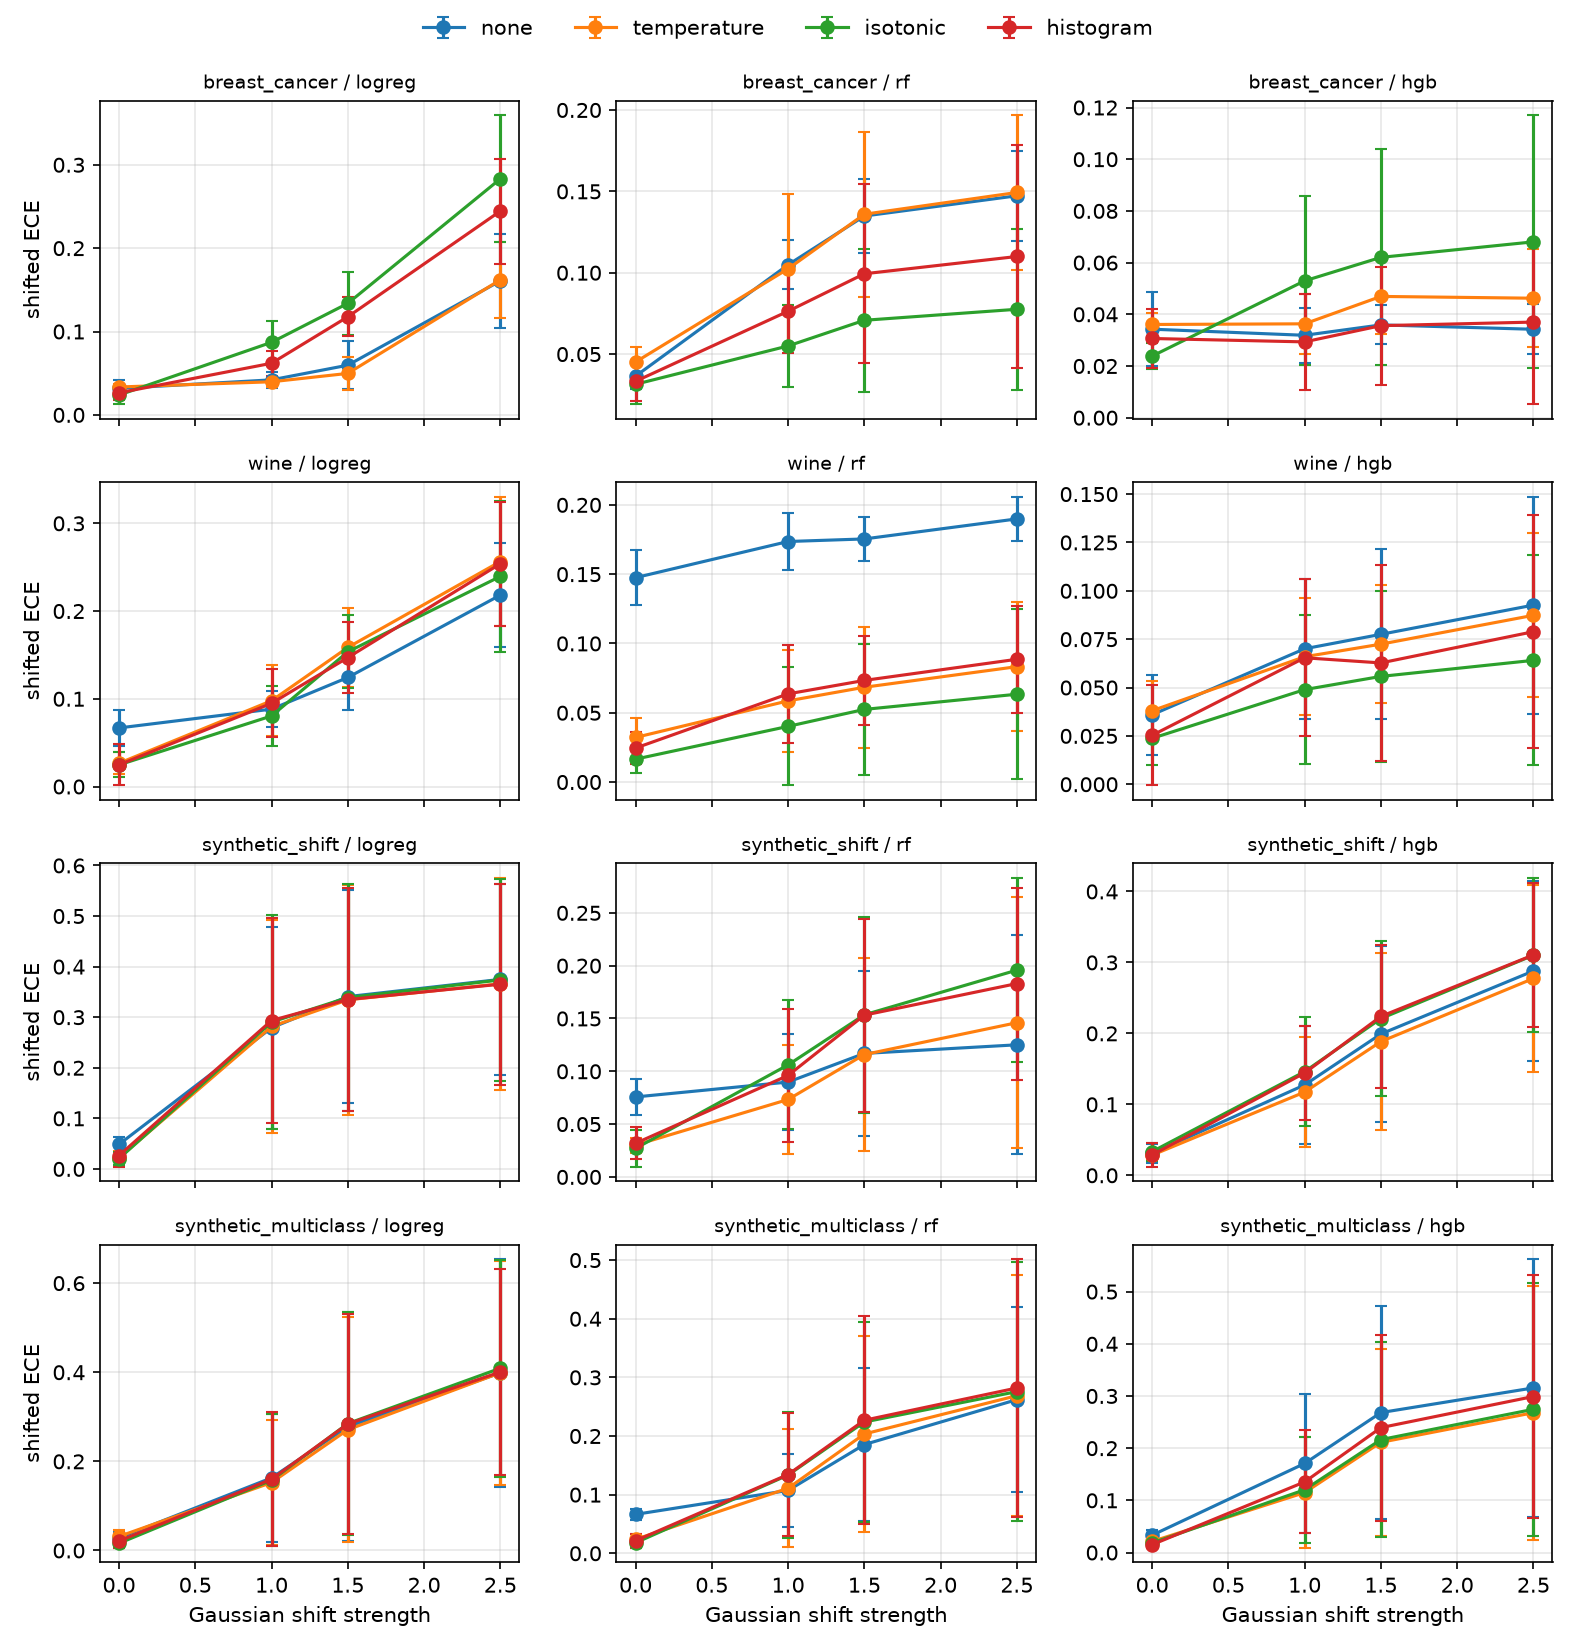
\includegraphics[width=\linewidth]{../figures/png/ece_vs_shift.png}
\caption{Shifted ECE vs.\ Gaussian feature-perturbation strength (mean
$\pm$ seed sd). $s{=}0$ is i.i.d.\ Labels are frozen; this is not
covariate shift. Source: \texttt{results/exp04\_main\_h1.json}.}
\label{fig:ece}
\end{figure}

\begin{figure}[t]
\centering
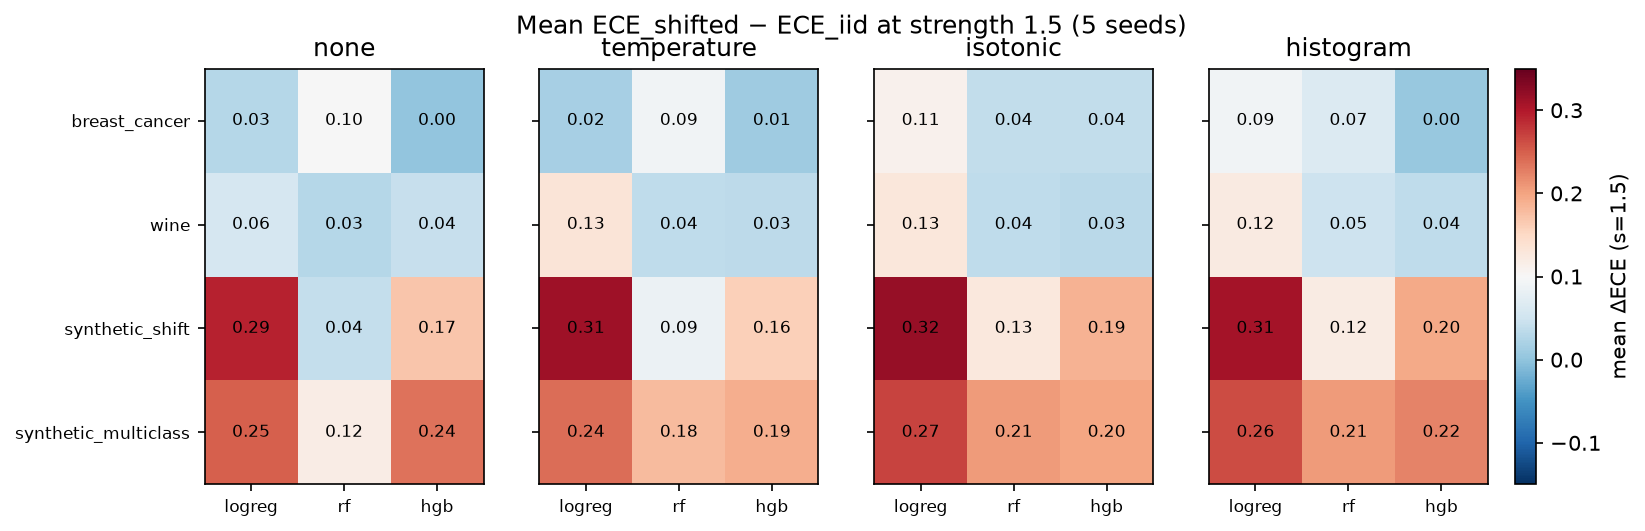
\includegraphics[width=\linewidth]{../figures/png/delta_ece_heatmap.png}
\caption{Mean $\Delta\mathrm{ECE}$ at $s{=}1.5$. Positive (red) means
the shifted test is \emph{worse} calibrated than the i.i.d.\ test.}
\label{fig:heat}
\end{figure}

\subsection{Post-hoc maps are not a reliable remedy}
Figure~\ref{fig:help} plots $\mathrm{ECE}_{\mathrm{shift}}(\mathrm{cal})-\mathrm{ECE}_{\mathrm{shift}}(\mathrm{none})$.
Wine random forests \emph{benefit} from isotonic
(\NumWineRfIsoHelp{} ECE; shifted ECE \NumWineRfNoneSh{} $\to$
\NumWineRfIsoSh), because the uncalibrated forest was already
badly calibrated. Temperature scaling on the same cell reaches shifted
ECE \NumWineRfTempSh. Breast-cancer logistic regression is \emph{hurt} by
isotonic (\NumBcLogregIsoHelp). We therefore do not rank calibrators under
shift.

\begin{figure}[t]
\centering
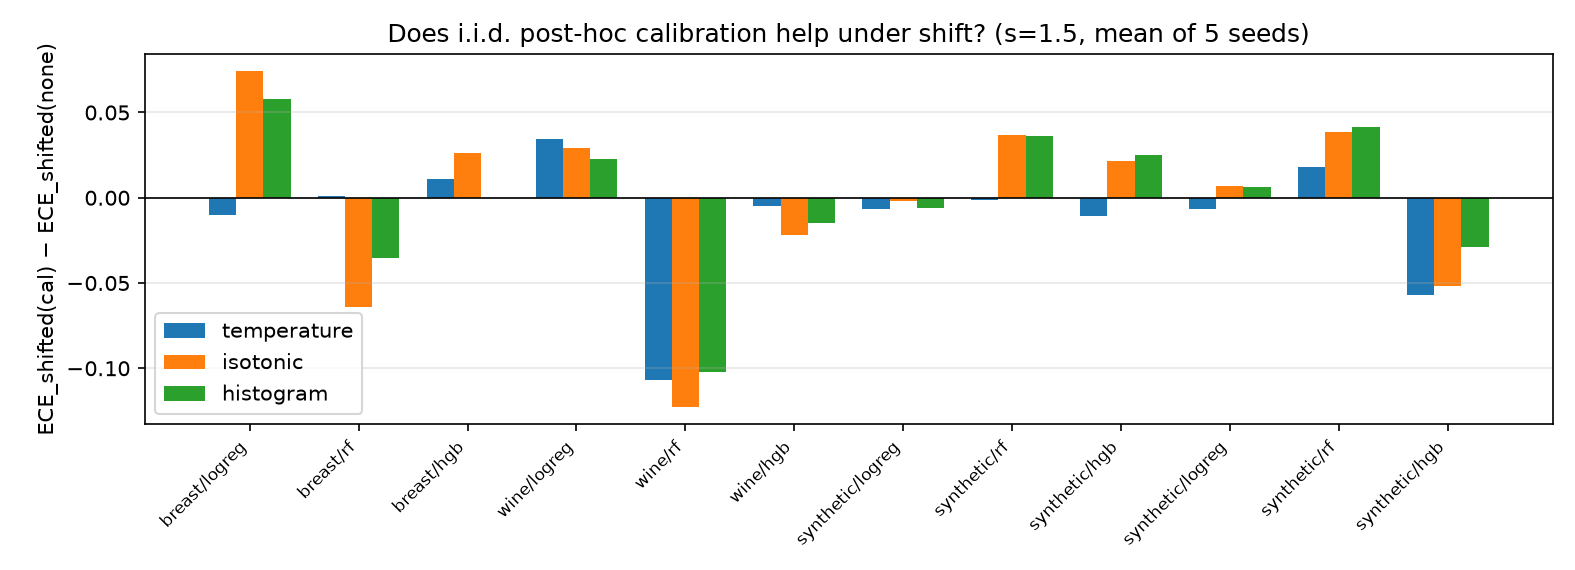
\includegraphics[width=\linewidth]{../figures/png/calibration_help_under_shift.png}
\caption{Does i.i.d.\ calibration help on the shifted test? Negative bars
mean the calibrator beats \texttt{none} under shift.}
\label{fig:help}
\end{figure}

\subsection{Coverage under perturbation}
Unweighted split conformal (logreg, \texttt{none}, LAC score $1-p_y$)
coverage at $\alpha=\NumAlpha$ (seed mean $\pm$ sd):
breast-cancer \NumBcLogregCovSZero$\pm$\NumBcLogregCovSZeroStd{} ($s{=}0$),
\NumBcLogregCovSOneFive$\pm$\NumBcLogregCovSOneFiveStd{} ($s{=}1.5$),
\NumBcLogregCovSTwoFive{} ($s{=}2.5$);
synthetic binary \NumSynthLogregCovSOneFive$\pm$\NumSynthLogregCovSOneFiveStd{}
at $s{=}1.5$ (Figure~\ref{fig:cov}). Exchangeability is broken by construction.
A 1-D ``oracle'' density ratio on feature $0$ did \emph{not}
restore coverage in the H3 pilot (killed).

\begin{figure}[t]
\centering
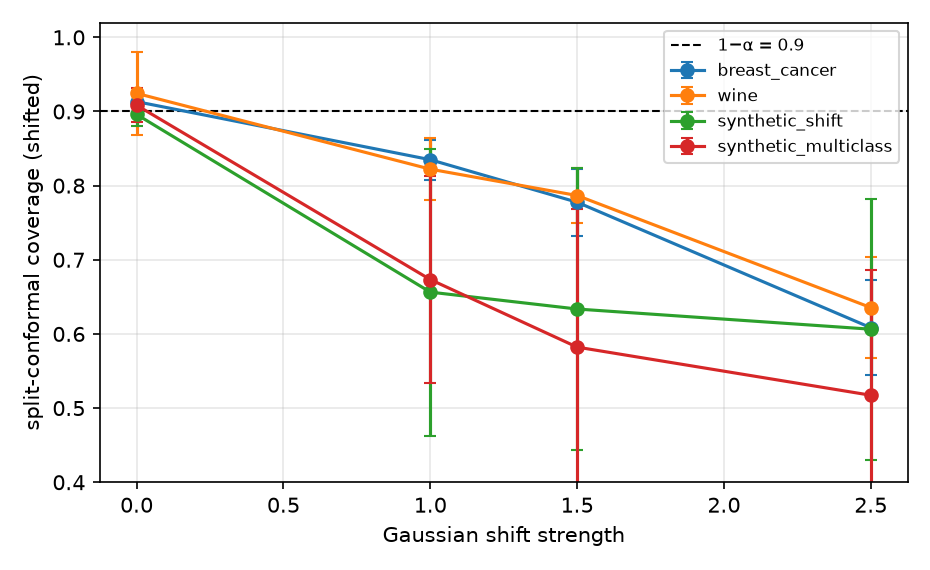
\includegraphics[width=\linewidth]{../figures/png/coverage_vs_shift.png}
\caption{Unweighted split-conformal coverage vs.\ feature perturbation
(logreg, no calibrator, LAC score). Dashed line: $1-\alpha=0.9$.}
\label{fig:cov}
\end{figure}

\subsection{Selection shift is a different, weaker effect}
Quantile slicing and importance resampling keep original $(X,y)$ pairs,
so $P(Y\mid X)$ is preserved and the mechanism is closer to covariate
shift. This ablation uses \NumExpFiveN{} dataset$\times$model cells on
\NumExpFiveNDs{} datasets (breast-cancer and
\texttt{synthetic\_shift}; wine and the multiclass synthetic are absent).
Mean $\Delta\mathrm{ECE}$ (\texttt{none}) is
\NumQuantileSliceDeltaMean{} (sd \NumQuantileSliceDeltaStd) for quantile
slice and \NumImpResampleDeltaMean{} (sd \NumImpResampleDeltaStd) for
importance resampling. On the \emph{same} \NumExpFiveN{} cells, Gaussian
perturbation at $s{=}1.5$ has cell-mean $\Delta\mathrm{ECE}$
\NumMatchedGaussDeltaMean{} (sd \NumMatchedGaussDeltaStd). Quantile slice
also moves accuracy less (cell-mean $\Delta$acc
\NumQuantileDeltaAccMean{} vs.\ matched Gaussian
\NumMatchedGaussDeltaAccMean), so the gap is not identified as
``preserving $P(Y\mid X)$'' alone. Importance resampling can even
\emph{decrease} ECE on breast-cancer. This control \textbf{does not
support} a claim that i.i.d.\ post-hoc calibration fails under covariate
shift in general.
Trailing-column perturbation on \texttt{synthetic\_shift} yields RF
$\Delta\mathrm{ECE}=\NumNoiseSynthRf$ vs.\ \NumPredSynthRf{} when
perturbing the first four columns.

\section{Limitations}
\begin{itemize}
\item \textbf{The headline mechanism is not covariate shift.} Frozen-label
feature mean-shift changes $P(Y\mid X)$ at the observed $x$ (input
corruption). Selection controls that preserve pairings show small
$\Delta\mathrm{ECE}$. Title and abstract are scoped accordingly.
\item \textbf{Shift is synthetic} and, for feature perturbation, entangled
with accuracy drop (synthetic logreg
\NumSynthLogregAccIid$\to$\NumSynthLogregAccShifted{} at $s{=}1.5$).
\item \textbf{Small tabular data only.} Wine test splits have
\NumWineNTest{} points and \NumWineNCal{} calibration points with
\NumEceBins{} ECE bins; those cells are noisy. No ImageNet, no LMs,
no naturally occurring drift (no Folktables/WILDS).
\item \textbf{Multiclass isotonic/histogram} map confidence, not a full
Dirichlet map \cite{kull2019dirichlet}; argmax can flip after
renormalization.
\item \textbf{Temperature on probabilities.} Trees have no logits; RF
$0/1$ probabilities saturate after clipping. This is not Guo logit
temperature.
\item \textbf{H3 weights were misspecified.} A 1-D histogram ratio is not
$p_{\mathrm{test}}(x)/p_{\mathrm{cal}}(x)$ for a 4-D perturbation.
\item \textbf{Pooling and tests.} Seed-level $n=\NumNoneN$ Wilcoxon is
pseudo-replicated and one-sided. The $n=\NumTwelveMeanN$ seed-averaged
uncalibrated means are a sign count, not independent replicates. A
dataset-level one-sided sign test has $n=\NumDatasetSignN$ and
$p{=}$\NumDatasetSignP. \NumNTests{} tests, unadjusted. Selection
comparisons use \NumExpFiveN{} cells on \NumExpFiveNDs{} datasets and
are not strength-matched to $s{=}1.5$ perturbation.
\item \textbf{Planar peg-in-hole cartoon, not a robot.} Dual-regime
numbers are from \texttt{exp09\_peg\_insert} (HistGradientBoosting,
\NumDualNSeeds{} seeds). Geometric clearance only: no MuJoCo, no DexNet,
no delayed-label receding calibrator in the homogeneous grid. Pre-registered
kill criteria fired: \texttt{\NumDualKillsFired}.
\item \textbf{Search scope.} Novelty is relative to
\texttt{paper/verified.bib}.
\end{itemize}

\section{Dual-regime insert/abort}
The tabular measurement says i.i.d.\ maps fail under frozen-label
perturbation, not under pairing-preserving selection. A hiring-relevant
task is whether that split changes \emph{what the agent does}, with
asymmetric cost: a false-confident insert is much worse than deferring
or aborting ($u_{\mathrm{wrong}}{=}-10$, $u_{\mathrm{correct}}{=}1$,
$u_{\mathrm{defer}}{=}-0.2$, $u_{\mathrm{abort}}{=}-0.5$).

We use a planar peg-in-hole cartoon (\texttt{src/dualregime/}). True
success is geometric clearance: $\mathrm{hypot}(x,y)+k|\theta|\le r_{\mathrm{clear}}$.
The deployed model sees encoder pose plus an unused appearance channel.
Camera pose is a watchdog, not a training feature. \emph{Optimistic
encoder bias} scales encoder $(x,y)$ toward the origin and freezes $Y$;
near-origin poses exist in training, so a PCA residual on encoder
coordinates \emph{falls} and is the wrong detection channel.
\emph{Selection} keeps pairs with $x\ge 0$ (right-half fixture). Success
rates are difficulty-matched (\NumDualPosIid{} i.i.d.\ vs.\
\NumDualPosSel{} slice).

Two channels, opposite legal moves. Physics residual
(encoder$-$camera, plus $\|p(\mathrm{raw})-p(\mathrm{projected})\|_1$)
routes to \textbf{project} the encoder onto the camera pose, then apply
source temperature and unweighted LAC: act if the set is $\{\mathrm{success}\}$,
else defer; abort only if residual is huge. Density ratio on camera
$xy$ (a domain classifier, not the killed 1-D feature-$0$ H3 estimator)
routes to the \emph{same} source $T$ plus multivariate weighted LAC:
act or \textbf{defer}, never abort-as-sensor-fault, never project as if
the encoder lied. Applying source $T$ to raw corrupted encoder
probabilities is an ablation (\texttt{illegal\_T} / \texttt{detector\_off}),
not the perturbation policy.

Figure~\ref{fig:dual}--\ref{fig:dualfcar} and
\texttt{results/summary\_dual.json} (\NumDualNSeeds{} seeds, HGB).
Under encoder bias, router mean utility is \NumPertRouterUtil{} vs.\
illegal raw-$T$ \NumPertIllegalUtil{} vs.\ abort-all
\NumPertAbortUtil{} vs.\ denoise-off (abort, no project)
\NumPertDenoiseOffUtil. FCAR drops from \NumPertIllegalFcr{} to
\NumPertRouterFcr; insert rate remains \NumPertRouterAct{} (abort rate
\NumPertRouterAbort, the huge-residual tail). Oracle/always-project
utility is \NumPertOracleUtil{}: the small gap is that tail, not a
second camera classifier. On i.i.d.\ tests the router does not pay a
large tax (\NumIidRouterUtil{} vs.\ \NumIidIidUtil). On the fixture
slice, abort rate is \NumSelRouterAbort{} and utility
\NumSelRouterUtil{} beats abort-all (\NumSelAbortUtil). Weighted
conformal does not have to \emph{help} here; it is enough that we do
not treat selection as a broken encoder. Mixed-stream blocks
(Figure~\ref{fig:dualstream}) keep those moves: slice-block density
label rate \NumStreamSelPredS, bias-block residual label rate
\NumStreamPertPredP, project-then-$T$ rate \NumStreamPertProj.
Kill criteria fired: \texttt{\NumDualKillsFired}. This is a kinematic
cartoon, not hardware \cite{luo2021conformal}.

\begin{figure}[t]
\centering
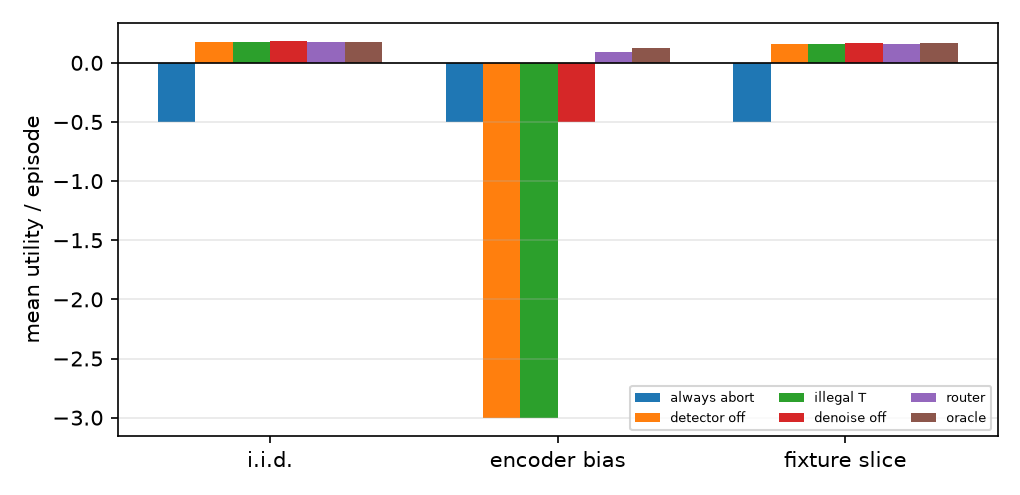
\includegraphics[width=\linewidth]{../figures/png/dual_regime_utility.png}
\caption{Mean insert/abort utility by test split and policy
(\NumDualNSeeds{} seeds). Optimistic encoder bias is not a fixture slice.}
\label{fig:dual}
\end{figure}

\begin{figure}[t]
\centering
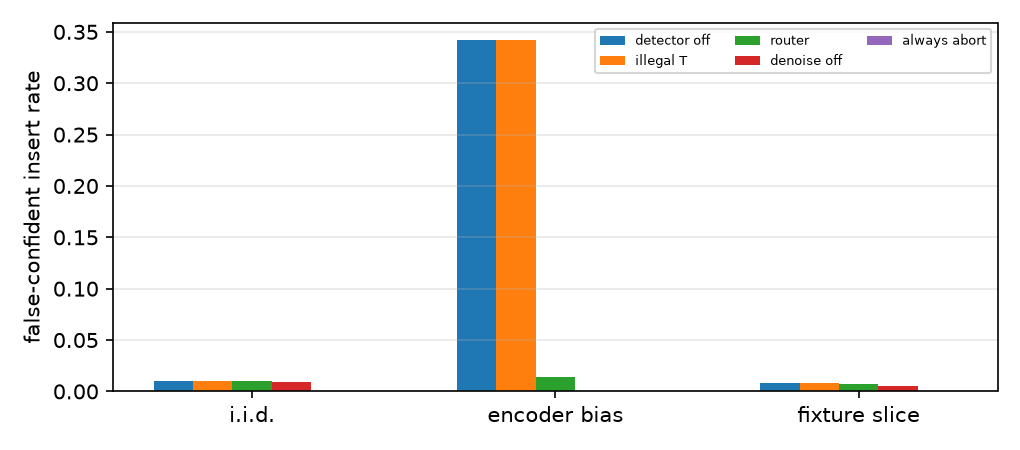
\includegraphics[width=\linewidth]{../figures/png/dual_regime_fcar.png}
\caption{False-confident insert rate. Source $T$ on raw encoder
probabilities is the incident; projecting then applying $T$ is not
abort-all.}
\label{fig:dualfcar}
\end{figure}

\begin{figure}[t]
\centering
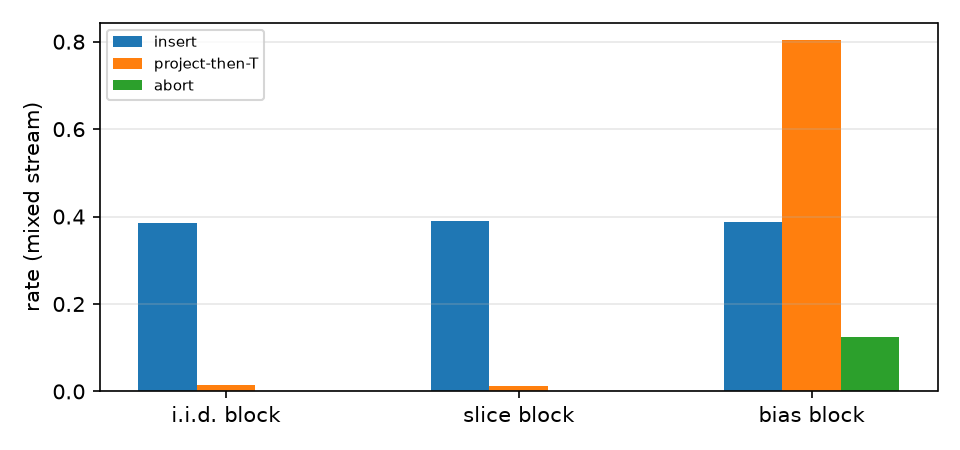
\includegraphics[width=\linewidth]{../figures/png/dual_regime_stream.png}
\caption{Mixed stream (i.i.d.\ then slice then encoder bias). Rolling
window; not one batch over the concatenated stream.}
\label{fig:dualstream}
\end{figure}

\section{Conclusion}
I.i.d.\ post-hoc maps are not a dependable answer to frozen-label
feature perturbation on these sklearn models, and they are not a
dependable \emph{insert} policy when the deployed encoder is the
sensor that moved. A residual channel that projects onto the camera
pose recovers utility under that perturbation and is not equivalent to
abort-all or to temperature scaling on raw corrupted probabilities.
Pairing-preserving selection is a different mechanism and a different
legal move (defer, not abort). The HGB exception and the killed H2/H3
hypotheses remain part of the tabular measurement.

\section*{AI-generation disclosure}
This repository and draft were produced by a coding agent executing the
user's \texttt{GOAL.md} protocol (literature verification via arXiv and
Semantic Scholar APIs, experiments on CPU, no hand-edited
\texttt{results/*.json}). Every numeric macro in \texttt{paper/numbers.tex}
is generated from those files. Citations are restricted to
\texttt{paper/verified.bib}. A human should still read the limitations
and re-run \texttt{make fresh-clone-test} before treating the PDF as
camera-ready.

\bibliographystyle{unsrtnat}
\bibliography{verified}
\end{document}
